\documentclass[journal]{IEEEtran}
\usepackage{amsmath,amssymb,amsfonts}
\usepackage{booktabs}
\usepackage{graphicx}
\usepackage{cite}
\usepackage{url}
\usepackage{multirow}
\usepackage{array}
\usepackage{color}

\newtheorem{proposition}{Proposition}

\graphicspath{{../figures/}}

\begin{document}

\title{Separating Viewer Motion from 3D Model Registration for Video See-Through Navigation}

\author{Ranyang~Li,
        Nan~Wei,
        Zhipeng~Lin,
        Wufeng~Liu,
        Chao~Fan,
        and~Junjun~Pan%
\thanks{This work was supported in part by the National Natural Science Foundation of China under Grant 62402163; in part by the Open Project Program of the State Key Laboratory of Virtual Reality Technology and Systems under Grant VRLAB2023C03; in part by the High-Level Talents Fund of Henan University of Technology under Grants 2022BS076 and 2022BS075; and in part by the Cultivation Project of the Tuoxin Team at Henan University of Technology under Grant 2024TXTD18. \emph{(Corresponding authors: Ranyang Li; Junjun Pan.)}}%
\thanks{Ranyang Li, Wufeng Liu, and Chao Fan are with the School of Artificial Intelligence and Big Data, Henan University of Technology, Zhengzhou 450001, China (e-mail: lry@haut.edu.cn).}%
\thanks{Nan Wei is with Henan Provincial People's Hospital, Zhengzhou University, Zhengzhou 450003, China.}%
\thanks{Zhipeng Lin and Junjun Pan are with the State Key Laboratory of Virtual Reality Technology and Systems, Beihang University, Beijing 100191, China (e-mail: linzhi\_p@outlook.com; pan\_junjun@buaa.edu.cn).}%
}

\markboth{IEEE Transactions on Visualization and Computer Graphics}{}

\maketitle

\begin{abstract}
Registering a 3D navigation model onto a live video see-through stream fails when the camera rotates rapidly, even when the physical target moves smoothly. Because the observed model-to-camera pose $T_{cm}$ composes the world-to-camera transformation $T_{cw}$ with the model-to-world transformation $T_{wm}$, temporal filtering on $T_{cm}$ misinterprets camera rotation as 3D target motion, while rendering with the exposure-time pose leaves an uncompensated pixel shift across the pipeline delay $\tau$. Pure 2D rotational image warps (Asynchronous TimeWarp) also break down at close working distances where camera translation and independent target motion induce depth parallax. We present a viewer-decoupled 3D registration method built on an inertial-guided static-anchor network (\emph{EgoAnchorNet}) and a two-stage temporal architecture. At frame exposure midpoint $t_e$, EgoAnchorNet subtracts the IMU-predicted rotational flow so stationary background pixels collapse to a translational epipolar field, separating static scene anchors ($99.1\%$ IoU) from moving targets ($88.9\%$ IoU) and driving cascaded differentiable Gauss--Newton solvers for both $T_{cw}(t_e)$ and $T_{wm}(t_e)$. At display completion $t_d = t_e + \tau$, the scene-referenced model pose $T_{wm}(t_e)$ is held fixed while only the viewer pose $T_{cw}$ is propagated across $\tau$ via the rigidly mounted IMU. In a three-condition counterfactual ablation across nine classical and learned methods (SIFT, ORB, KLT, LoFTR, RAFT, ATW, VGGT, Reloc3r, and Pi3), removing viewer ego-motion cuts fast-turn ($[2.0,10.0)$~rad/s) target-region rotation error by $43.4\%\text{--}77.8\%$ and AR overlay drift from $42.1$~px ($52.4$~px under 2D ATW) to $10.2$~px. In direct head-to-head evaluation under simultaneous camera and target motion, EgoAnchorNet achieves $0.08^\circ$ median camera rotation error and $1.31^\circ$ target rotation error at $68.2$~ms per pair, outperforming VGGT ($1.82^\circ$, $165$~ms), Pi3 ($2.01^\circ$, $95$~ms), and Reloc3r ($2.24^\circ$, $118$~ms), while reducing high-rate 3D model Average Distance (ADD) error to $1.79\text{--}2.19$~mm.
\end{abstract}

\begin{IEEEkeywords}
Video see-through augmented reality, 3D model registration, static-anchor motion disentanglement, viewer motion compensation, camera-IMU fusion, angular-velocity stratification.
\end{IEEEkeywords}

\begin{figure*}[!t]
\centering
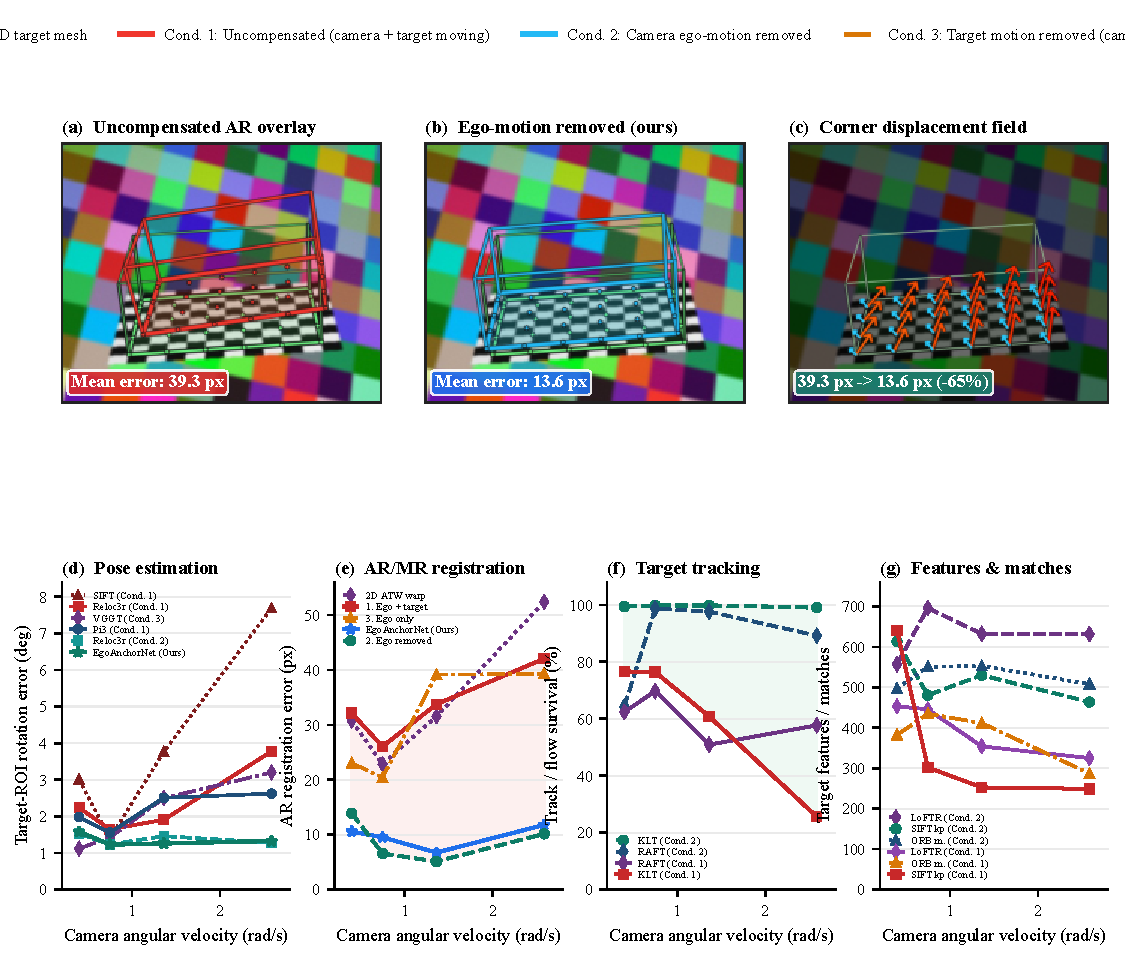
\includegraphics[width=\textwidth]{intro_relative_motion.pdf}
\caption{Three-condition counterfactual ablation under simultaneous camera and target motion ($1280\times720$, shared aggressive 6DoF camera trajectory, $10$ pairs per angular-velocity bin). \textbf{(a)} Uncompensated AR overlay (Condition~1: camera and target both moving at $3.40$~rad/s); the 3D navigation prism (red) shifts by $39.3$~px from the ground-truth target mesh (green). \textbf{(b)} Camera ego-motion removed (Condition~2), leaving only the target's single-frame motion ($13.6$~px, cyan). \textbf{(c)} Corner displacement field ($39.3$~px $\rightarrow$ $13.6$~px, $-65\%$). \textbf{(d)} Median rotation error in the $360\times210$ target region of interest (ROI) for Pi3~\cite{wang2025pi3}, Reloc3r~\cite{dong2025reloc3r}, VGGT~\cite{wang2025vggt}, SIFT~\cite{lowe2004distinctive}, and EgoAnchorNet (Ours). \textbf{(e)} AR registration error across Condition~1 (ego + target), Condition~3 (ego only, target fixed), 2D Asynchronous TimeWarp (ATW)~\cite{lu2025quasar,gao2025xrgo}, EgoAnchorNet Stage-I, and Condition~2 (Stage-II ego removed). \textbf{(f)} Pyramidal Lucas--Kanade~\cite{lucas1981iterative} and dense RAFT~\cite{teed2020raft} survival on the target. \textbf{(g)} Detector-free LoFTR~\cite{sun2021loftr} matches, SIFT keypoints, and ORB~\cite{rublee2011orb} matches on the target.}
\label{fig:intro}
\end{figure*}

\section{Introduction}
\IEEEPARstart{V}{ideo} see-through augmented reality (AR) navigation overlays a pre-reconstructed 3D model---such as a computed tomography (CT) organ mesh or a computer-aided design (CAD) target---directly onto live video frames captured by a 4K camera or a stereo endoscope~\cite{higgins2013continuous,bernhardt2017status,ishihara2023integrating}. Unlike optical see-through head-mounted displays (HMDs), the display is the video frame itself, and both the handheld or robot-mounted camera and the physical target move in 3D space while surrounding background structures remain stationary. Whenever the camera rotates rapidly, the rendered 3D overlay detaches from the physical target.

This failure stems from how registration pipelines represent and update the composite model-to-camera transformation
\begin{equation}
T_{cm}(t) = T_{cw}(t)\,T_{wm}(t) \in \mathrm{SE}(3),
\label{eq:comp}
\end{equation}
where $T_{cw}(t)$ maps world coordinates into the camera frame and $T_{wm}(t)$ places the 3D model in the scene. Treating $T_{cm}(t)$ as a single state variable creates three compounding errors under viewer motion. First, in the image plane, camera rotation $\boldsymbol{\omega}$ sweeps every pixel by approximately $f\|\boldsymbol{\omega}\|\Delta t$ regardless of depth $z$, masking the boundary between stationary background regions ($\mathcal{M}_{\text{stat}}$) and the independently moving target ($\mathcal{M}_{\text{obj}}$). Second, in 3D pose estimation, any correspondence or optical-flow solver that does not strictly isolate $\mathcal{M}_{\text{stat}}$ leaks target motion into the camera ego-motion estimate $T_{cw}(t)$, while temporal smoothing on the composite pose $T_{cm}(t)$ projects camera acceleration onto the 3D model trajectory. Third, over the pipeline latency $\tau = t_d - t_e$ between exposure midpoint $t_e$ and display write $t_d$, rendering with $T_{cm}(t_e)$ leaves an uncompensated rotational swim $f\|\boldsymbol{\omega}\|\tau$, whereas 2D post-rendering warps such as Asynchronous TimeWarp (ATW)~\cite{lincoln2016motion,lu2025quasar,gao2025xrgo} fail at close working distances ($z \approx 150$~mm) where camera translation and target displacement violate the zero-parallax homography assumption.

To determine whether high-rate registration failure is driven by target dynamics or by viewer ego-motion, we first conduct a three-condition counterfactual ablation in which both ground-truth camera trajectory $T_{wc}(t)$ and independent target trajectory $T_{wm}(t)$ are controlled (Fig.~\ref{fig:intro}): Condition~1 retains both camera and target 6DoF motion; Condition~2 removes viewer ego-motion while preserving the exact 3D target trajectory $T_{wm}(t)$; and Condition~3 freezes the target in world space while replaying the exact camera trajectory $T_{wc}(t)$ (or extrapolates the coupled pose $T_{cm}$). Across nine classical and learned baselines---SIFT~\cite{lowe2004distinctive}, ORB~\cite{rublee2011orb}, Lucas--Kanade (KLT)~\cite{lucas1981iterative}, LoFTR~\cite{sun2021loftr}, RAFT~\cite{teed2020raft}, 2D ATW~\cite{lu2025quasar}, VGGT~\cite{wang2025vggt}, Reloc3r~\cite{dong2025reloc3r}, and Pi3~\cite{wang2025pi3}---Condition~1 and Condition~3 degrade together in the $[2.0,10.0)$~rad/s bin, whereas removing viewer ego-motion in Condition~2 restores dense matches ($+77.0\%\text{--}94.3\%$) and tracking survival ($89.2\%\text{--}99.0\%$), cuts target-ROI rotation error by $43.4\%\text{--}77.8\%$, and reduces AR overlay shift from $42.1$~px ($52.4$~px under 2D ATW) to $10.2$~px.

We resolve both the spatial and temporal coupling between viewer and target motion through an inertial-guided static-anchor network (\emph{EgoAnchorNet}) and a two-stage registration architecture. At the exposure midpoint $t_e$, EgoAnchorNet uses the preintegrated rotation increment $\Delta R_{\text{imu}}$ from a rigidly mounted IMU to subtract depth-independent rotational optical flow, reducing stationary background flow to a pure translational epipolar field that separates $\mathcal{M}_{\text{stat}}$ from $\mathcal{M}_{\text{obj}}$. Cascaded differentiable Gauss--Newton solvers then estimate $T_{cw}(t_e)$ strictly on $\mathcal{M}_{\text{stat}}$ and $T_{wm}(t_e)$ on the camera-subtracted residual flow of $\mathcal{M}_{\text{obj}}$. Temporal filtering acts on the scene-referenced pose $T_{wm}(t_e) = T_{cw}(t_e)^{-1}T_{cm}(t_e)$, and at display time $t_d = t_e + \tau$, only the viewer pose $T_{cw}$ is propagated across $\tau$ via the IMU. Our contributions are threefold:
\begin{enumerate}
    \item \textbf{Inertial De-Rotated Static-Anchor Disentanglement and Cascaded Dual-$\mathrm{SE}(3)$ Solver (\emph{EgoAnchorNet}):} We introduce an inertial de-rotation operator that removes rotational flow before motion segmentation, isolating stationary scene anchors ($99.1\%$ IoU) from moving targets ($88.9\%$ IoU) and driving cascaded differentiable Gauss--Newton solvers that jointly recover metric camera ego-motion ($0.08^\circ$ median rotation error) and 3D target motion ($1.31^\circ$ median rotation error).
    \item \textbf{Two-Stage Viewer-Decoupled Registration and Display-Time Compensation Architecture:} We decouple exposure-time scene-coordinate filtering on $T_{wm}(t_e)$ from display-time IMU propagation on $T_{cw}(t_d)$, preventing viewer acceleration from corrupting the 3D model state while eliminating depth-invariant rotational swim over $\tau$.
    \item \textbf{Counterfactual Dual-Motion Benchmark and Angular-Velocity-Stratified Verification:} We build a hybrid benchmark pairing 6DoF dual-motion ground truth with real endoscopic textures from SCARED~\cite{allan2021scared}, evaluate nine classical/learned baselines and four network ablations across four angular-velocity bins, and verify $1.79\text{--}2.19$~mm 3D model ADD accuracy across 4K+IMU and stereo+IMU setups.
\end{enumerate}

\section{Related Work}
We group prior work by the failure modes that occur when a 3D model is registered to a live video stream under viewer motion, and list open-source implementations in Table~\ref{tab:code}.

\subsection{Display Latency and View Reprojection in AR and Graphics}
Post-rendering reprojection updates a rendered image to match viewer motion between rendering and display. Lincoln et al.~\cite{lincoln2016motion} reduced motion-to-photon latency on an optical see-through HMD to $80~\mu\text{s}$ using low-persistence modulation and 2D post-render warps at $50^\circ/\text{s}$ head turns. For video see-through HMDs, Ishihara et al.~\cite{ishihara2023integrating} combined eye-camera parallax warping with latency compensation ($50\text{--}62.5$~ms uncompensated delay), and Wang et al.~\cite{wang2024vicomp} compensated geometric and radiometric delay in projector-camera systems (ViComp).

In recent ACM SIGGRAPH and XR runtime systems, Lu and Rowe~\cite{lu2025quasar} introduced QUASAR (SIGGRAPH 2025), which streams pixel-aligned quad geometry rather than 2D frames so a client can reproject views under 6DoF motion with motion parallax and disocclusion handling, releasing open-source baselines for Asynchronous TimeWarp (ATW, $H = K R_{\text{new}}^{-1} R_{\text{old}} K^{-1}$), MeshWarp, and QuadStream. Gao et al.~\cite{gao2025xrgo} developed XRgo and OpenWarp (integrated into ILLIXR) for 6DoF mesh and raymarching reprojection, while Yang et al.~\cite{yang2024mobfgsr} (Mob-FGSR, SIGGRAPH 2024) used motion-vector frame extrapolation to hide rendering latency on mobile GPUs.

Two properties prevent these display-warping methods from solving video see-through 3D model registration: (i) rotational 2D warps (ATW) assume zero translation or infinite depth, which fails at close working distances ($z \approx 150$~mm) where camera translation and independent target motion produce large parallax ($52.4$~px ATW error in Fig.~\ref{fig:intro}(e)); and (ii) all of them assume the virtual object's 3D pose in the scene is already known, so they do not prevent an upstream pose filter on $T_{cm}$ from absorbing viewer rotation.

\begin{table}[!t]
\centering
\caption{Open-Source Repositories for Latency Reprojection, Dynamic Motion Decoupling, and Correspondence Estimation.}
\label{tab:code}
\renewcommand{\arraystretch}{1.10}
\resizebox{\columnwidth}{!}{%
\begin{tabular}{llll}
\toprule
\textbf{System} & \textbf{Venue} & \textbf{Scope} & \textbf{GitHub Repository} \\
\midrule
ViComp~\cite{wang2024vicomp} & TVCG 24 & Proj.-cam warp & \texttt{cyxwang/ViComp} \\
OpenWarp~\cite{gao2025xrgo} & MMSys 25 & 6DoF XR warp & \texttt{Zee2/openwarp} \\
QUASAR~\cite{lu2025quasar} & SIGGRAPH 25 & Quad / ATW warp & \texttt{quasar-gfx/QUASAR} \\
PAD3R~\cite{liao2025pad3r} & SIGGRAPH Asia 25 & Offline 4D recon. & \texttt{pad3r/pad3r-public} \\
Shape of Motion~\cite{wang2025shape} & ICCV 25 & Offline 4D tracks & \texttt{vye16/shape-of-motion} \\
MegaSaM~\cite{li2025megasam} & CVPR 25 & Dynamic video BA & \texttt{mega-sam/mega-sam} \\
BA-Track~\cite{chen2025batrack} & ICCV 25 & Decoupled 3D BA & \texttt{wrchen530/batrack} \\
VGGT~\cite{wang2025vggt} & CVPR 25 & Feed-forward 3D & \texttt{facebookresearch/vggt} \\
Reloc3r~\cite{dong2025reloc3r} & CVPR 25 & Pairwise pose & \texttt{ffrivera0/reloc3r} \\
Pi3~\cite{wang2025pi3} & arXiv 25 & Equivariant pose & \texttt{yyfz/Pi3} \\
LoFTR~\cite{sun2021loftr} & CVPR 21 & Dense matcher & \texttt{zju3dv/LoFTR} \\
RAFT~\cite{teed2020raft} & ECCV 20 & Recurrent flow & \texttt{princeton-vl/RAFT} \\
OpenVINS~\cite{geneva2020openvins} & ICRA 20 & Stereo-IMU VIO & \texttt{rpng/open\_vins} \\
XR-Check~\cite{hu2025xr} & ISMAR 25 & XR tracking bench. & \texttt{Duke-I3T-Lab/XR\_Tracking\_Evaluation} \\
\bottomrule
\end{tabular}%
}
\end{table}

\subsection{Decoupling Camera Ego-Motion from Dynamic Objects}
Separating camera-induced pixel motion from independent object motion has been studied in recent SIGGRAPH and computer vision pipelines. At SIGGRAPH Asia 2025, Liao et al.~\cite{liao2025pad3r} proposed PAD3R, which reconstructs deformable 3D objects from casual monocular videos by pairing a DINOv2 camera pose estimator with CoTracker3 2D correspondences. Wang et al.~\cite{wang2025shape} (Shape of Motion) and Li et al.~\cite{li2025megasam} (MegaSaM) recover camera trajectories in dynamic videos by masking or down-weighting moving foreground regions during differentiable bundle adjustment. Chen et al.~\cite{chen2025batrack} (BA-Track) decompose observed 3D point tracks into a camera-induced component and a dynamic-object component so epipolar bundle adjustment can retain both static and moving points.

For online correspondence and pose estimation, detector-free transformer matchers such as LoFTR~\cite{sun2021loftr} and recurrent optical-flow networks such as RAFT~\cite{teed2020raft} replace hand-crafted descriptors (SIFT~\cite{lowe2004distinctive}, ORB~\cite{rublee2011orb}) and local Lucas--Kanade tracking~\cite{lucas1981iterative}. Feed-forward 3D foundation models---including DUSt3R~\cite{wang2024dust3r}, VGGT~\cite{wang2025vggt}, Reloc3r~\cite{dong2025reloc3r}, and Pi3~\cite{wang2025pi3}---regress relative poses directly from image pairs, while visual-inertial odometry (VIO) systems such as OpenVINS~\cite{geneva2020openvins}, Basalt~\cite{usenko2020basalt}, ORB-SLAM3~\cite{campos2021orbslam3}, and collaborative mobile AR SLAM~\cite{pan2024collaborative} fuse camera tracks with IMU preintegration.

However, three gaps remain when applying these methods to live 3D model registration:
\begin{enumerate}
    \item Offline 4D optimization pipelines (PAD3R~\cite{liao2025pad3r}, Shape of Motion~\cite{wang2025shape}, MegaSaM~\cite{li2025megasam}, BA-Track~\cite{chen2025batrack}) require multi-pass global optimization over full video sequences rather than causal frame-by-frame execution within a $33\text{--}70$~ms budget.
    \item When a moving target occupies the navigation ROI, feed-forward pose networks (VGGT~\cite{wang2025vggt}, Pi3~\cite{wang2025pi3}, Reloc3r~\cite{dong2025reloc3r}) and dense matchers/trackers (LoFTR~\cite{sun2021loftr}, RAFT~\cite{teed2020raft}) suffer from viewer-induced blur and perspective foreshortening (Fig.~\ref{fig:intro} and Table~\ref{tab:ablation}).
    \item Lightweight single-pose flow solvers (such as baseline coupled EgoLite) assign non-zero weight to deforming or moving regions and solve only for camera ego-motion, leaving the moving target's 3D trajectory unestimated and allowing target motion to bias camera translation.
\end{enumerate}

\subsection{3D Model Registration in Endoscopic and Camera Navigation}
In surgical and industrial navigation, a prior 3D model (CT/MRI mesh or CAD model) is aligned to live video~\cite{higgins2013continuous,bernhardt2017status}. Continuous bronchoscopy and laparoscopy registration systems~\cite{higgins2013continuous,bernhardt2017status} report that fast scope rotation causes blur and overlay swim, forcing operators to pan slowly or restricting overlays to static keyframes. Public endoscopic datasets such as SCARED~\cite{allan2021scared} and EndoSLAM~\cite{ozyoruk2021endoslam} lack synchronized camera-mounted IMU streams paired with controlled angular-velocity tiers and independent target motion ground truth; furthermore, poses in ray-cast synthetic sets are often derived from 2D--3D registration itself, making them circular for causal evaluation. Recent ISMAR benchmarks on spatial tracking~\cite{hu2025xr,lima2025hololens}, 3D reconstruction alignment (MR-Compare~\cite{zhu2026mrcompare}), and perceptual registration ambiguity~\cite{lu2026registration} confirm that session-averaged trajectory metrics conceal high-velocity failures and that registration offsets beyond task tolerance cause users to select the wrong target. We therefore evaluate both 3D millimetre error and 2D pixel shift directly against IMU angular velocity.

\begin{figure*}[!t]
\centering
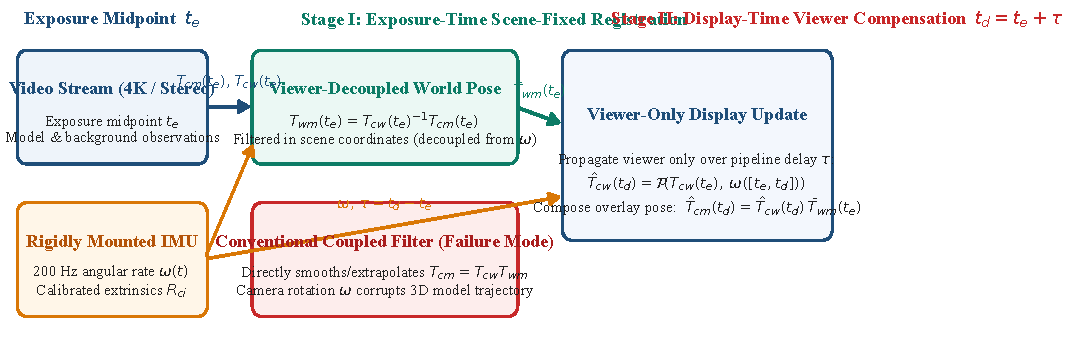
\includegraphics[width=\textwidth]{fig2_two_stage_architecture.pdf}
\caption{Two-stage viewer-decoupled registration architecture. At the exposure midpoint $t_e$ (Stage~I), the measured composite pose $T_{cm}(t_e)$ is mapped to scene coordinates via $T_{cw}(t_e)^{-1}$ so filtering acts on $T_{wm}(t_e)$ without absorbing camera angular velocity $\boldsymbol{\omega}$. At display completion $t_d = t_e + \tau$ (Stage~II), only the viewer pose $T_{cw}$ is propagated across the measured pipeline delay $\tau$ using the rigidly mounted IMU.}
\label{fig:arch}
\end{figure*}

\section{Methodology}
\subsection{Coordinate Frames, Notation, and Preliminaries}
We define four right-handed 3D coordinate frames: the stationary world (scene) frame $\mathcal{F}_w$, the moving camera frame $\mathcal{F}_c$ (with $+X$ right, $+Y$ down, and $+Z$ along the optical axis), the rigidly mounted IMU frame $\mathcal{F}_i$, and the local coordinate frame $\mathcal{F}_m$ of the 3D navigation model. A rigid transformation $T_{ab} = (R_{ab}, \mathbf{p}_{ab}) \in \mathrm{SE}(3)$ with rotation $R_{ab} \in \mathrm{SO}(3)$ and translation $\mathbf{p}_{ab} \in \mathbb{R}^3$ maps a homogeneous point $\mathbf{X}_b \in \mathbb{R}^3$ from $\mathcal{F}_b$ to $\mathcal{F}_a$ via $\mathbf{X}_a = R_{ab}\mathbf{X}_b + \mathbf{p}_{ab}$. Specifically, $T_{cw}(t) = T_{wc}(t)^{-1}$ denotes the world-to-camera pose, $T_{wm}(t)$ denotes the model-to-world pose, $T_{cm}(t) = T_{cw}(t)T_{wm}(t)$ denotes the composite model-to-camera pose, and $R_{ci} \in \mathrm{SO}(3)$ is the calibrated camera-from-IMU extrinsic rotation.

For a twist vector $\boldsymbol{\xi} = [\boldsymbol{\rho}^\top, \boldsymbol{\theta}^\top]^\top \in \mathbb{R}^6$ with translational component $\boldsymbol{\rho} \in \mathbb{R}^3$ and rotational component $\boldsymbol{\theta} \in \mathbb{R}^3$, the hat operator $[\cdot]_\times : \mathbb{R}^3 \rightarrow \mathfrak{so}(3)$ produces the skew-symmetric matrix $[\boldsymbol{\theta}]_\times$, and $\exp_{\mathrm{SE}(3)}(\boldsymbol{\xi}^\wedge)$ and $\log_{\mathrm{SE}(3)}(T)$ denote the matrix exponential and logarithm between $\mathfrak{se}(3)$ and $\mathrm{SE}(3)$. Given camera intrinsics $K \in \mathbb{R}^{3\times 3}$ with focal lengths $(f_x, f_y)$ and principal point $(c_x, c_y)$, the perspective projection of a 3D point $\mathbf{X}_c = [X, Y, Z]^\top \in \mathcal{F}_c$ onto pixel coordinates $\mathbf{u} = [u, v]^\top \in \mathbb{R}^2$ is $\mathbf{u} = \Pi(K\mathbf{X}_c)$, where $\Pi([x, y, z]^\top) = [x/z, y/z]^\top$.

\subsection{Image-Plane Drift over the Pipeline Delay}
Let $\mathbf{X}_m \in \mathcal{F}_m$ be a vertex on the 3D model. Over the pipeline delay $\tau = t_d - t_e$ between frame exposure midpoint $t_e$ and completed overlay write $t_d$, the camera moves by the left increment
\begin{equation}
\Delta T_{c}(t_e, t_d) = T_{cw}(t_d)\,T_{cw}(t_e)^{-1} = \exp_{\mathrm{SE}(3)}\!\left(\begin{bmatrix}\boldsymbol{\rho}\\ \boldsymbol{\theta}\end{bmatrix}^\wedge\right),
\end{equation}
with rotation vector $\boldsymbol{\theta} \approx \boldsymbol{\omega}\,\tau$ induced by camera angular velocity $\boldsymbol{\omega} \in \mathbb{R}^3$ and translation $\boldsymbol{\rho} \approx \mathbf{v}\,\tau$ induced by linear velocity $\mathbf{v} \in \mathbb{R}^3$. For mean focal length $f = \frac{1}{2}(f_x+f_y)$ and target depth $z$, rendering at $t_d$ with the exposure-time pose $T_{cm}(t_e)$ produces a first-order pixel shift
\begin{align}
\Delta u_{\text{drift}}(\tau) &\approx \underbrace{f\,\|\boldsymbol{\omega}\|\,\tau}_{\text{viewer rotation}} + \underbrace{\frac{f\,\|\mathbf{v}\|\,\tau}{z}}_{\text{viewer translation}} \nonumber\\
&\quad + \underbrace{\Delta u_{\text{target}}(\tau)}_{\text{target motion}}.
\label{eq:drift}
\end{align}
At $f = 1095$~px ($1280\times720$) and $\tau = 60$~ms, a $2.6$~rad/s camera turn yields $171$~px of rotational shift regardless of depth $z$, exceeding the target's own single-frame displacement $\Delta u_{\text{target}}(\tau)$.

\subsection{EgoAnchorNet: Inertial-Guided Static-Anchor Dual-$\mathrm{SE}(3)$ Solver}
In a scene partitioned into stationary background pixels $\mathcal{M}_{\text{stat}}$ ($\mathbf{X}_w(t_{e,k}) = \mathbf{X}_w(t_{e,k-1})$) and independently moving target pixels $\mathcal{M}_{\text{obj}}$ ($\mathbf{X}_w(t_{e,k}) = R_{B}\mathbf{X}_w(t_{e,k-1}) + \mathbf{p}_B$), a 3D point $\mathbf{X}_{c,k-1} = Z(\mathbf{u})\,K^{-1}\tilde{\mathbf{u}}$ (where $\tilde{\mathbf{u}} = [u, v, 1]^\top$ and $Z(\mathbf{u}) > 0$ is metric depth) transforms between frames $t_{e,k-1}$ and $t_{e,k}$ as
\begin{equation}
\mathbf{X}_{c,k}(\mathbf{u}) = \begin{cases}
\Delta R_{\text{cam}}\,\mathbf{X}_{c,k-1}(\mathbf{u}) + \Delta\mathbf{t}_{\text{cam}}, & \mathbf{u} \in \mathcal{M}_{\text{stat}}, \\[4pt]
\Delta R_{\text{obj}}\,\mathbf{X}_{c,k-1}(\mathbf{u}) + \Delta\mathbf{t}_{\text{obj}}, & \mathbf{u} \in \mathcal{M}_{\text{obj}},
\end{cases}
\label{eq:3d_motion_piecewise}
\end{equation}
where $(\Delta R_{\text{cam}}, \Delta\mathbf{t}_{\text{cam}}) \in \mathrm{SE}(3)$ is the camera relative motion and $(\Delta R_{\text{obj}}, \Delta\mathbf{t}_{\text{obj}}) \in \mathrm{SE}(3)$ is the composite target-in-camera relative motion.

\subsubsection{Inertial De-Rotation and Translational Epipolar Reduction}
From a single image pair, raw optical flow $\mathbf{f}_{\text{obs}}(\mathbf{u}) = \Pi(K\mathbf{X}_{c,k}(\mathbf{u})) - \mathbf{u}$ is dominated by camera rotation $\Delta R_{\text{cam}}$, which sweeps all pixels across the image plane regardless of whether they belong to $\mathcal{M}_{\text{stat}}$ or $\mathcal{M}_{\text{obj}}$ (Fig.~\ref{fig:ego_anchor}(a)). Using the preintegrated IMU rotation increment $\Delta R_{\text{imu}} = \exp_{\mathrm{SO}(3)}([R_{ci}\boldsymbol{\omega}_{i}\Delta t]_\times)$, we compute the pure rotational flow
\begin{equation}
\mathbf{f}_{\text{rot}}(\mathbf{u}; \Delta R_{\text{imu}}) = \Pi\!\left(K\,\Delta R_{\text{imu}}\,K^{-1}\tilde{\mathbf{u}}\right) - \mathbf{u},
\label{eq:f_rot}
\end{equation}
and subtract it from $\mathbf{f}_{\text{obs}}(\mathbf{u})$ to form the de-rotated flow field
\begin{equation}
\mathbf{f}_{\text{rot-free}}(\mathbf{u}) = \mathbf{f}_{\text{obs}}(\mathbf{u}) - \mathbf{f}_{\text{rot}}(\mathbf{u}; \Delta R_{\text{imu}}).
\label{eq:rot_free}
\end{equation}

\begin{proposition}[Translational Epipolar Reduction on Static Anchors]
\label{prop:epipolar}
Assume calibrated IMU-to-camera rotation $\Delta R_{\text{imu}} = \Delta R_{\text{cam}}$. For any stationary anchor pixel $\mathbf{u} \in \mathcal{M}_{\text{stat}}$ with rotated depth $Z'(\mathbf{u}) = \mathbf{e}_3^\top(\Delta R_{\text{cam}}\mathbf{X}_{c,k-1}(\mathbf{u}) + \Delta\mathbf{t}_{\text{cam}})$, the de-rotated flow $\mathbf{f}_{\text{rot-free}}(\mathbf{u})$ is independent of camera rotation on rays where $Z(\mathbf{u}) \gg |\Delta t_z|$ and satisfies the exact radial focus-of-expansion constraint
\begin{equation}
\mathbf{f}_{\text{rot-free}}(\mathbf{u}) = \frac{1}{Z'(\mathbf{u})} \begin{bmatrix} f_x & 0 & u_{\text{rot}} - c_x \\ 0 & f_y & v_{\text{rot}} - c_y \end{bmatrix} \begin{bmatrix} \Delta t_{\text{cam},x} \\ \Delta t_{\text{cam},y} \\ -\Delta t_{\text{cam},z} \end{bmatrix},
\label{eq:foe_exact}
\end{equation}
where $\mathbf{u}_{\text{rot}} = [u_{\text{rot}}, v_{\text{rot}}]^\top = \Pi(K\Delta R_{\text{cam}}K^{-1}\tilde{\mathbf{u}})$. Conversely, for any moving target pixel $\mathbf{u} \in \mathcal{M}_{\text{obj}}$ with non-zero world motion $(R_B, \mathbf{p}_B) \neq (I_3, \mathbf{0})$, $\mathbf{f}_{\text{rot-free}}(\mathbf{u})$ deviates from Eq.~\eqref{eq:foe_exact} by the target-induced flow residual $\Delta\mathbf{f}_{\text{obj}}(\mathbf{u}) \neq \mathbf{0}$.
\end{proposition}

\begin{IEEEproof}
For $\mathbf{u} \in \mathcal{M}_{\text{stat}}$, let $\mathbf{X}_{\text{rot}} = \Delta R_{\text{cam}}\mathbf{X}_{c,k-1}(\mathbf{u}) = Z(\mathbf{u})\Delta R_{\text{cam}}K^{-1}\tilde{\mathbf{u}} = [X_r, Y_r, Z_r]^\top$. By projective scale invariance, $\Pi(K\mathbf{X}_{\text{rot}}) = \Pi(K\Delta R_{\text{cam}}K^{-1}\tilde{\mathbf{u}}) = \mathbf{u}_{\text{rot}}$, so $X_r/Z_r = (u_{\text{rot}}-c_x)/f_x$ and $Y_r/Z_r = (v_{\text{rot}}-c_y)/f_y$. Substituting $\mathbf{X}_{c,k}(\mathbf{u}) = \mathbf{X}_{\text{rot}} + \Delta\mathbf{t}_{\text{cam}}$ with $Z'(\mathbf{u}) = Z_r + \Delta t_{\text{cam},z}$ into $\mathbf{f}_{\text{rot-free}}(\mathbf{u}) = \Pi(K\mathbf{X}_{c,k}(\mathbf{u})) - \mathbf{u}_{\text{rot}}$ yields
\begin{align}
f_{\text{rot-free},u}(\mathbf{u}) &= \frac{f_x(X_r + \Delta t_{\text{cam},x})}{Z_r + \Delta t_{\text{cam},z}} - (u_{\text{rot}} - c_x) \nonumber\\
&= \frac{f_x \Delta t_{\text{cam},x} - (u_{\text{rot}} - c_x)\Delta t_{\text{cam},z}}{Z'(\mathbf{u})},
\end{align}
and identically for $f_{\text{rot-free},v}(\mathbf{u})$, which gives Eq.~\eqref{eq:foe_exact}. Thus all rays $\mathbf{u} \in \mathcal{M}_{\text{stat}}$ point away from (or toward) the single translational epipole $\mathbf{e}_{\text{cam}} = \Pi(K\Delta\mathbf{t}_{\text{cam}})$. For $\mathbf{u} \in \mathcal{M}_{\text{obj}}$, $\Delta R_{\text{obj}} = R_{c,k}^\top R_B R_{c,k-1} \neq \Delta R_{\text{cam}}$ or $\Delta\mathbf{t}_{\text{obj}} \neq \Delta\mathbf{t}_{\text{cam}}$, violating Eq.~\eqref{eq:foe_exact}.
\end{IEEEproof}

Guided by Proposition~\ref{prop:epipolar}, we feed image features $(F_0, F_{1\leftarrow 0}, |F_0 - F_{1\leftarrow 0}|)$, observed flow $\mathbf{f}_{\text{obs}}$, and de-rotated flow features $(\mathbf{f}_{\text{rot-free}}, \|\mathbf{f}_{\text{rot-free}}\|)$ on a $1/8$-resolution grid ($32\times 40$) into a dilated residual decoder to predict: (i) static-anchor probability $p_{\text{stat}}(\mathbf{u}) \in [0,1]$ and moving-target probability $p_{\text{obj}}(\mathbf{u}) = 1 - p_{\text{stat}}(\mathbf{u})$; (ii) branch-specific flow log-variances $(\log\sigma_c^2(\mathbf{u}), \log\sigma_o^2(\mathbf{u}))$; and (iii) metric depth $Z(\mathbf{u}) = Z_{\text{nom}}\exp(r(\mathbf{u}))$ in millimetres ($Z_{\text{nom}} = 150$~mm).

\subsubsection{Cascaded Dual-$\mathrm{SE}(3)$ Differentiable Gauss--Newton Solvers}
Unlike baseline EgoLite---which blends moving regions into the camera solver via a positive weight share and solves only a single camera pose---EgoAnchorNet enforces strict zero-contamination gating between two cascaded Gauss--Newton solvers:
\begin{enumerate}
    \item \emph{Camera Ego-Motion Solver on Static Anchors:} Using weights $w_{\text{stat}}(\mathbf{u}) = p_{\text{stat}}(\mathbf{u})^2 \exp(-\log\sigma_c^2(\mathbf{u}))$ that vanish on $\mathcal{M}_{\text{obj}}$, we minimize the Huber-reweighted ($\rho_H$) static flow objective coupled with the IMU rotational prior ($\lambda_{\text{imu}} = 400$):
    \begin{align}
    \min_{\Delta R_{\text{cam}}, \Delta\mathbf{t}_{\text{cam}}} &\sum_{\mathbf{u}} w_{\text{stat}}(\mathbf{u})\,\rho_H\!\Big(\big\|\mathbf{f}_{\text{obs}}(\mathbf{u}) - \mathbf{f}_{\text{cam}}(\mathbf{u})\big\|^2\Big) \nonumber\\
    &+ \lambda_{\text{imu}}\,\big\|\log_{\mathrm{SO}(3)}\!\big(\Delta R_{\text{imu}}\,\Delta R_{\text{cam}}^\top\big)\big\|^2.
    \label{eq:solve_cam}
    \end{align}
    \item \emph{Target 3D Motion Solver on Isolated Residual Flow:} Evaluating $\mathbf{f}_{\text{cam}}(\mathbf{u}; Z, \Delta R_{\text{cam}}, \Delta\mathbf{t}_{\text{cam}})$ across the full grid and subtracting it from $\mathbf{f}_{\text{obs}}$ isolates the target's non-zero motion field $\mathbf{f}_{\text{iso}}(\mathbf{u}) = \mathbf{f}_{\text{obs}}(\mathbf{u}) - \mathbf{f}_{\text{cam}}(\mathbf{u})$ (Fig.~\ref{fig:ego_anchor}(d)). A second differentiable Gauss--Newton solver weighted by $w_{\text{obj}}(\mathbf{u}) = p_{\text{obj}}(\mathbf{u})^2 \exp(-\log\sigma_o^2(\mathbf{u}))$ then solves for the target's 3D relative transformation $(\Delta R_{\text{obj}}, \Delta\mathbf{t}_{\text{obj}})$:
    \begin{equation}
    \min_{\Delta R_{\text{obj}}, \Delta\mathbf{t}_{\text{obj}}} \sum_{\mathbf{u}} w_{\text{obj}}(\mathbf{u})\,\rho_H\!\Big(\big\|\mathbf{f}_{\text{obs}}(\mathbf{u}) - \mathbf{f}_{\text{obj}}(\mathbf{u})\big\|^2\Big).
    \label{eq:solve_obj}
    \end{equation}
\end{enumerate}
A closed-loop refinement module then concatenates the post-solve residuals $\mathbf{r}_c = \mathbf{f}_{\text{obs}} - \mathbf{f}_{\text{cam}}$ and $\mathbf{r}_o = \mathbf{f}_{\text{obs}} - \mathbf{f}_{\text{obj}}$ with the decoder features to update $(p_{\text{stat}}, \log\sigma_c^2, \log\sigma_o^2)$ and run two additional Gauss--Newton iterations for both branches.

\subsection{Two-Stage Scene-Fixed Filtering and Display Update}
Given exposure-midpoint measurements, filtering $\tilde{T}_{cm}$ directly feeds the coupled innovation
\begin{align}
\boldsymbol{\xi}_{cm,k} &= \log_{\mathrm{SE}(3)}\!\left(\tilde{T}_{cm,k-1}^{-1}\,\tilde{T}_{cm,k}\right) \nonumber\\
&= \log_{\mathrm{SE}(3)}\!\left(T_{wm,k-1}^{-1}\,(T_{cw,k-1}^{-1}T_{cw,k})\,T_{wm,k}\right),
\label{eq:coupled_xi}
\end{align}
which mixes camera motion $T_{cw,k-1}^{-1}T_{cw,k}$ into the model update.

In Stage~I (Fig.~\ref{fig:arch}), we remove the exposure-time viewer pose $T_{cw}(t_{e,k})$ before smoothing:
\begin{equation}
\tilde{T}_{wm}(t_{e,k}) = T_{cw}(t_{e,k})^{-1}\,\tilde{T}_{cm}(t_{e,k}),
\label{eq:world_lift}
\end{equation}
and update the scene-referenced model pose $\bar{T}_{wm}(t_{e,k})$ on $\mathrm{SE}(3)$:
\begin{align}
\bar{T}_{wm}(t_{e,k}) &= \bar{T}_{wm}(t_{e,k-1})\nonumber\\
&\quad \cdot \exp_{\mathrm{SE}(3)}\!\Big(\mathcal{G}\big(\log_{\mathrm{SE}(3)}(\bar{T}_{wm,k-1}^{-1}\tilde{T}_{wm,k})\big)\Big),
\label{eq:world_filter}
\end{align}
where $\mathcal{G}(\cdot)$ is the filter gain operator.

In Stage~II, at display time $t_d = t_e + \tau$, $\bar{T}_{wm}(t_{e,k})$ is held fixed in the scene while only the viewer pose is propagated over $[t_e, t_d]$ using IMU angular velocity $\boldsymbol{\omega}_i(t)$ and calibrated camera-to-IMU rotation $R_{ci}$:
\begin{equation}
\hat{T}_{cw}(t_d) = \mathcal{P}\!\left(T_{cw}(t_e),\,\{R_{ci}\boldsymbol{\omega}_i(t)\}_{t\in[t_e, t_d]},\,\tau\right),
\label{eq:viewer_prop}
\end{equation}
and the display overlay pose is composed as
\begin{equation}
\hat{T}_{cm}(t_d) = \hat{T}_{cw}(t_d)\,\bar{T}_{wm}(t_e).
\label{eq:render_pose}
\end{equation}

\section{Experimental Setup and Hybrid Dataset}
\subsection{Hardware Platforms and Hybrid R2S Dual-Motion Corpus}
We evaluate two physical camera-IMU configurations and a hybrid dual-motion benchmark:
\begin{enumerate}
    \item \textbf{Device A (4K Camera + IMU):} A monocular 4K camera ($3840\times2160$ sensor output; intrinsics scaled to $1280\times720$, $512\times288$, and $320\times256$ for registration inference) rigidly mounted with a $200$~Hz 6-axis USB IMU. The camera-to-IMU rotation $R_{ci}$ is calibrated via rigid hand-eye alignment:
    \[
    R_{ci} = \begin{bmatrix}
    0.007668 & -0.946526 & -0.322536 \\
    -0.003137 & 0.322521 & -0.946557 \\
    0.999966 & 0.008270 & -0.000496
    \end{bmatrix}.
    \]
    Millimetre error on the monocular 4K setup uses a known target length ($12\times9$ inner grid, $3.0$~mm square size).
    \item \textbf{Device B (Stereo Endoscope Configuration + IMU):} A stereo endoscopic camera pair ($1280\times720$ per eye, $30$~fps, nominal baseline $b = 46.5$~mm in simulation, to be replaced by wet-lab stereo calibration before clinical use) paired with a $200$~Hz IMU noise model fitted from static USB recordings. Stereo disparity defines metric scale in millimetres, and exposure-midpoint IMU gyroscope readings define $\|\boldsymbol{\omega}\|$.
    \item \textbf{Hybrid Dual-Motion + Static-Anchor Corpus:} To train and evaluate EgoAnchorNet with exact pixel-level stationarity labels and independent 6DoF poses for both camera and target, we generate $1{,}125$ dual-motion pairs ($865$ training across $24$ sequences, $260$ validation across $8$ sequences, plus $40$ held-out test pairs across $4$ angular-velocity bins). Half of the sequences texture the stationary background surface with real porcine abdominal cavity keyframes from SCARED~\cite{allan2021scared} (datasets 5--7), while the target object executes independent 6DoF spline trajectories ($\pm 20\text{--}32$~mm translation, $14^\circ\text{--}24^\circ$ rotation, $95$th-percentile speed $79.1$~mm/s) and the camera executes aggressive 6DoF trajectories ($\pm 40$~mm translation, $10^\circ\text{--}24^\circ$ rotation) without tracking the target. Each pair provides exact $32\times 40$ metric depth maps, binary static-anchor masks $\mathcal{M}_{\text{stat}}$, noisy $200$~Hz IMU preintegrated rotations $\Delta R_{\text{imu}}$, and ground-truth $(\Delta R_{\text{cam}}, \Delta\mathbf{t}_{\text{cam}})$ and $(\Delta R_{\text{obj}}, \Delta\mathbf{t}_{\text{obj}})$.
\end{enumerate}

\subsection{Timing, Hardware, and Angular-Velocity Bins}
Experiments run on an NVIDIA RTX~5090 Laptop GPU (24~GB VRAM) with distributed verification on RTX~3080 (16~GB) and GTX~1070 (8~GB) nodes. EgoAnchorNet is trained for $8$ epochs using AdamW ($\text{lr}=3\times 10^{-4}$, cosine schedule, batch size $8$, $290$~s wall-clock training time). Pipeline delay $\tau$ is timed on one clock from exposure midpoint $t_e$ to overlay completion $t_d$, covering both single-frame intervals ($\Delta t = 33.3$~ms at $30$~fps) and full pipeline latency ($\tau = 60.0$~ms, pose estimation included). Frames and pairs are partitioned into four IMU angular-velocity bins:
\begin{align*}
\mathcal{B}_1 &= [0.0,0.5),\quad \mathcal{B}_2 = [0.5,1.0),\\
\mathcal{B}_3 &= [1.0,2.0),\quad \mathcal{B}_4 = [2.0,10.0)\text{~rad/s}.
\end{align*}
To ensure statistical rigor across skewed and heavy-tailed error distributions, we report both non-parametric **Median [Interquartile Range, IQR]** and parametric **Mean $\pm$ Standard Deviation (SD)**.

\section{Results}

\begin{table*}[!t]
\centering
\caption{Unified Head-to-Head Benchmark and Three-Condition Counterfactual Ablation Across Classical, SOTA Learned, and Proposed Methods Stratified by Camera Angular Velocity ($1280\times720$, $10$ Pairs per Bin, $N=40$ Total; Values Reported as \textbf{Median [IQR]} / Mean $\pm$ SD).}
\label{tab:ablation}
\renewcommand{\arraystretch}{1.12}
\resizebox{\textwidth}{!}{%
\begin{tabular}{lllcccccc}
\toprule
\textbf{Task / Metric} & \textbf{Method} & \textbf{Condition / Setting} & \textbf{$\mathcal{B}_1: [0.0, 0.5)$} & \textbf{$\mathcal{B}_2: [0.5, 1.0)$} & \textbf{$\mathcal{B}_3: [1.0, 2.0)$} & \textbf{$\mathcal{B}_4: [2.0, 10.0)$} & \textbf{All Bins ($N=40$)} & \textbf{Time} \\
\midrule
\multirow{11}{*}{\textbf{1. Pose Error ($^\circ$)}} 
 & SIFT~\cite{lowe2004distinctive} + Essential & Cond.~1: Ego + Target & 3.00 [7.50] / 21.4$\pm$49.5 & 1.40 [1.67] / 3.93$\pm$5.63 & 3.76 [19.5] / 16.0$\pm$22.7 & 7.69 [7.40] / 40.6$\pm$69.0 & 3.13 [8.49] / 20.5$\pm$46.0 & 42 ms \\
 & Reloc3r~\cite{dong2025reloc3r} (CVPR'25) & Cond.~1: Ego + Target & 2.24 [1.27] / 2.61$\pm$1.74 & 1.65 [1.84] / 1.33$\pm$0.98 & 1.91 [1.19] / 2.08$\pm$1.33 & 3.78 [2.10] / 4.22$\pm$1.55 & 2.24 [1.56] / 2.56$\pm$1.78 & 118 ms \\
 & Pi3~\cite{wang2025pi3} (2025) & Cond.~1: Ego + Target & 1.98 [1.02] / 2.43$\pm$2.10 & 1.56 [1.02] / 1.39$\pm$0.87 & 2.51 [1.67] / 2.11$\pm$0.84 & 2.62 [1.48] / 2.89$\pm$1.03 & 2.01 [1.59] / 2.21$\pm$1.43 & 95 ms \\
 & VGGT~\cite{wang2025vggt} (CVPR'25) & Cond.~1: Ego + Target & 2.51 [1.38] / 2.32$\pm$1.41 & 1.60 [1.28] / 2.32$\pm$2.05 & 1.80 [1.07] / 1.91$\pm$0.66 & 1.94 [2.43] / 2.59$\pm$1.26 & 1.82 [1.32] / 2.29$\pm$1.46 & 165 ms \\
 & VGGT~\cite{wang2025vggt} (CVPR'25) & Cond.~3: Ego Only & 1.12 [0.82] / 1.26$\pm$1.27 & 1.42 [3.10] / 2.17$\pm$1.62 & 2.50 [1.64] / 2.84$\pm$1.69 & 3.20 [2.18] / 15.5$\pm$36.2 & 1.88 [2.64] / 5.44$\pm$19.1 & 165 ms \\
 & Coupled EgoLite & Cond.~1: Ego + Target & 1.46 [0.87] / 1.61$\pm$0.72 & 1.23 [0.45] / 1.22$\pm$0.38 & 1.36 [0.52] / 1.35$\pm$0.46 & 1.48 [0.34] / 1.46$\pm$0.41 & 1.40 [0.52] / 1.41$\pm$0.53 & 54 ms \\
\cmidrule(lr){2-9}
 & SIFT~\cite{lowe2004distinctive} + Essential & Cond.~2: Ego Removed & 1.45 [3.61] / 20.8$\pm$53.1 & 3.80 [4.31] / 21.2$\pm$53.0 & 3.03 [2.95] / 3.54$\pm$1.81 & 1.71 [1.48] / 1.79$\pm$0.98 & 2.11 [3.90] / 11.8$\pm$38.6 & --- \\
 & VGGT~\cite{wang2025vggt} (CVPR'25) & Cond.~2: Ego Removed & 1.60 [0.96] / 1.67$\pm$0.76 & 1.37 [0.86] / 1.16$\pm$0.59 & 1.29 [0.36] / 1.30$\pm$0.68 & 1.81 [0.99] / 1.57$\pm$0.71 & 1.40 [0.92] / 1.43$\pm$0.72 & --- \\
 & Reloc3r~\cite{dong2025reloc3r} (CVPR'25) & Cond.~2: Ego Removed & 1.53 [1.06] / 1.27$\pm$0.69 & 1.23 [0.90] / 1.10$\pm$0.58 & 1.46 [1.55] / 1.18$\pm$0.82 & 1.28 [1.43] / 1.06$\pm$0.79 & 1.38 [1.10] / 1.15$\pm$0.73 & --- \\
 & Pi3~\cite{wang2025pi3} (2025) & Cond.~2: Ego Removed & 2.11 [0.54] / 1.75$\pm$0.92 & 1.65 [1.89] / 1.33$\pm$0.97 & 1.87 [1.70] / 1.29$\pm$0.91 & 0.96 [1.44] / 0.92$\pm$0.75 & 1.71 [2.11] / 1.32$\pm$0.94 & --- \\
 & \textbf{EgoAnchorNet (Ours, Target)} & \textbf{Cond.~1: Ego + Target} & \textbf{1.58 [0.78] / 1.61$\pm$0.67} & \textbf{1.23 [0.88] / 1.06$\pm$0.58} & \textbf{1.26 [0.19] / 1.19$\pm$0.54} & \textbf{1.33 [0.64] / 1.22$\pm$0.50} & \textbf{1.31 [0.63] / 1.27$\pm$0.61} & \textbf{68 ms} \\
 & \textbf{EgoAnchorNet (Ours, Camera)} & \textbf{Cond.~1: Ego + Target} & \textbf{0.09 [0.08] / 0.09$\pm$0.06} & \textbf{0.07 [0.04] / 0.07$\pm$0.03} & \textbf{0.07 [0.04] / 0.07$\pm$0.04} & \textbf{0.12 [0.07] / 0.12$\pm$0.06} & \textbf{0.08 [0.07] / 0.09$\pm$0.05} & \textbf{68 ms} \\
\midrule
\multirow{5}{*}{\textbf{2. AR Shift (px)}} 
 & Uncompensated Overlay & Cond.~1: Ego + Target & 32.1 [33.2] / 32.1$\pm$19.9 & 26.1 [16.4] / 22.6$\pm$10.1 & 33.8 [7.51] / 33.3$\pm$9.85 & 42.1 [6.40] / 42.5$\pm$5.82 & 33.6 [16.5] / 32.6$\pm$14.4 & --- \\
 & 2D ATW Warp~\cite{lu2025quasar,gao2025xrgo} & Cond.~1: Rot. Homog. & 30.7 [28.1] / 32.6$\pm$17.0 & 22.9 [11.8] / 26.6$\pm$14.2 & 31.6 [18.4] / 29.9$\pm$21.6 & 52.4 [37.2] / 54.6$\pm$24.1 & 32.2 [27.1] / 35.9$\pm$22.5 & $<1$ ms \\
 & Coupled EgoLite & Cond.~1: Ego + Target & 10.3 [7.73] / 14.0$\pm$10.9 & 12.8 [8.49] / 12.7$\pm$5.72 & 8.77 [6.28] / 9.83$\pm$4.77 & 15.0 [3.99] / 15.5$\pm$6.33 & 12.0 [8.30] / 13.0$\pm$7.61 & 54 ms \\
 & \textbf{EgoAnchorNet Stage-I (Ours)} & \textbf{Cond.~1: Ego + Target} & \textbf{10.6 [7.71] / 13.2$\pm$10.3} & \textbf{9.52 [6.29] / 11.4$\pm$4.35} & \textbf{6.74 [6.93] / 8.38$\pm$4.50} & \textbf{11.8 [12.9] / 16.4$\pm$14.4} & \textbf{9.79 [8.99] / 12.3$\pm$9.83} & \textbf{68 ms} \\
 & \textbf{Two-Stage Viewer-Decoupled} & \textbf{Cond.~2: Ego Removed} & \textbf{13.9 [9.51] / 10.9$\pm$5.87} & \textbf{6.58 [3.06] / 7.10$\pm$3.20} & \textbf{5.11 [3.68] / 6.68$\pm$3.90} & \textbf{10.2 [3.30] / 9.38$\pm$3.18} & \textbf{7.48 [7.65] / 8.52$\pm$4.53} & \textbf{$<1$ ms} \\
\midrule
\multirow{2}{*}{\textbf{3. 3D ADD (mm)}} 
 & Coupled EgoLite & Cond.~1: Ego + Target & 3.93 [3.93] / 3.68$\pm$2.12 & 2.86 [1.26] / 3.32$\pm$2.20 & 2.37 [3.35] / 3.40$\pm$2.40 & 3.70 [4.03] / 4.34$\pm$2.19 & 2.90 [3.91] / 3.68$\pm$2.26 & 54 ms \\
 & \textbf{EgoAnchorNet (Ours)} & \textbf{Cond.~1: Ego + Target} & \textbf{2.22 [1.58] / 2.51$\pm$1.35} & \textbf{2.08 [0.97] / 2.11$\pm$0.95} & \textbf{1.70 [0.75] / 1.64$\pm$0.55} & \textbf{1.79 [1.49] / 2.60$\pm$2.27} & \textbf{1.89 [1.10] / 2.21$\pm$1.48} & \textbf{68 ms} \\
\midrule
\multirow{5}{*}{\textbf{4. Tracking (\%)}} 
 & KLT~\cite{lucas1981iterative} Survival (\%) & Cond.~1: Ego + Target & 76.6 [18.3] / 78.0$\pm$14.6 & 76.4 [27.6] / 79.6$\pm$16.5 & 60.8 [14.8] / 64.0$\pm$18.2 & 25.6 [38.3] / 34.1$\pm$21.3 & 68.2 [27.2] / 63.9$\pm$25.5 & 6 ms \\
 & RAFT~\cite{teed2020raft} Survival (\%) & Cond.~1: Ego + Target & 62.4 [43.3] / 62.4$\pm$23.8 & 69.7 [34.5] / 65.8$\pm$23.0 & 50.9 [42.5] / 55.7$\pm$27.3 & 57.7 [45.3] / 54.0$\pm$26.6 & 60.1 [45.1] / 59.4$\pm$25.7 & 28 ms \\
 & \textbf{EgoAnchorNet Inliers (\%)} & \textbf{Cond.~1: Ego + Target} & \textbf{96.6 [11.6] / 94.0$\pm$6.76} & \textbf{94.2 [8.29] / 93.4$\pm$7.96} & \textbf{85.0 [22.4] / 83.7$\pm$13.8} & \textbf{68.7 [38.7] / 70.3$\pm$22.3} & \textbf{91.8 [22.3] / 85.4$\pm$17.1} & \textbf{68 ms} \\
 & RAFT~\cite{teed2020raft} Survival (\%) & Cond.~2: Ego Removed & 64.3 [54.8] / 69.2$\pm$26.4 & 98.7 [15.7] / 93.0$\pm$8.10 & 97.6 [11.4] / 93.1$\pm$9.07 & 89.2 [9.07] / 91.9$\pm$5.19 & 95.0 [15.7] / 86.8$\pm$17.9 & --- \\
 & KLT~\cite{lucas1981iterative} Survival (\%) & Cond.~2: Ego Removed & 99.4 [13.4] / 93.1$\pm$10.2 & 99.8 [0.43] / 97.5$\pm$4.80 & 99.8 [2.96] / 95.9$\pm$6.77 & 99.0 [2.05] / 98.2$\pm$2.41 & 99.6 [2.47] / 96.2$\pm$6.96 & --- \\
\midrule
\multirow{6}{*}{\textbf{5. Features / Match}} 
 & LoFTR~\cite{sun2021loftr} Matches & Cond.~1: Ego + Target & 453 [84.3] / 477$\pm$157 & 446 [88.5] / 446$\pm$142 & 354 [119] / 405$\pm$114 & 325 [115] / 306$\pm$99 & 394 [132] / 408$\pm$144 & 48 ms \\
 & LoFTR~\cite{sun2021loftr} Matches & Cond.~2: Ego Removed & \textbf{557 [145] / 618$\pm$159} & \textbf{696 [54.8] / 686$\pm$59} & \textbf{632 [242] / 664$\pm$151} & \textbf{632 [99.8] / 630$\pm$119} & \textbf{635 [153] / 649$\pm$130} & --- \\
 & SIFT~\cite{lowe2004distinctive} Keypoints & Cond.~1: Ego + Target & 641 [485] / 639$\pm$238 & 302 [113] / 291$\pm$82 & 253 [93.0] / 241$\pm$73 & 249 [67.3] / 231$\pm$47 & 290 [134] / 351$\pm$215 & 35 ms \\
 & SIFT~\cite{lowe2004distinctive} Keypoints & Cond.~2: Ego Removed & \textbf{614 [255] / 672$\pm$174} & \textbf{481 [57.3] / 484$\pm$38} & \textbf{530 [117] / 572$\pm$132} & \textbf{464 [79.8] / 481$\pm$53} & \textbf{521 [92.5] / 552$\pm$138} & --- \\
 & ORB~\cite{rublee2011orb} Matches & Cond.~1: Ego + Target & 382 [109] / 388$\pm$99 & 435 [74.3] / 423$\pm$47 & 412 [61.3] / 406$\pm$34 & 287 [59.5] / 300$\pm$58 & 385 [97.3] / 379$\pm$80 & 12 ms \\
 & ORB~\cite{rublee2011orb} Matches & Cond.~2: Ego Removed & \textbf{498 [40.8] / 499$\pm$30} & \textbf{551 [54.5] / 546$\pm$41} & \textbf{553 [65.0] / 539$\pm$49} & \textbf{508 [49.3] / 506$\pm$57} & \textbf{528 [68.8] / 523$\pm$49} & --- \\
\bottomrule
\end{tabular}%
}
\end{table*}

\begin{figure*}[!t]
\centering
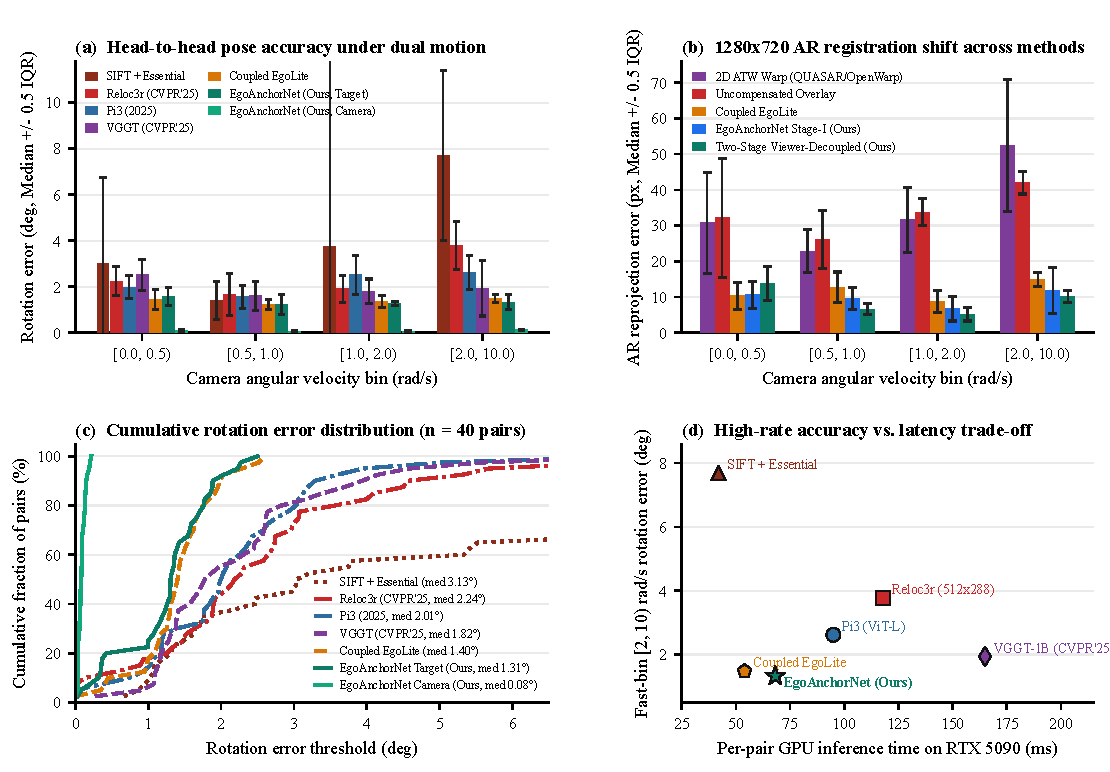
\includegraphics[width=\textwidth]{fig5_sota_head_to_head.pdf}
\caption{Head-to-head comparison of EgoAnchorNet and Two-Stage Viewer-Decoupled Registration against classical and SOTA baselines on the 40-pair dual-motion test benchmark. \textbf{(a)} Target-ROI rotation error (Median $\pm$ $0.5$~IQR) across the four angular-velocity bins. \textbf{(b)} $1280\times720$ AR reprojection error (px, Median $\pm$ $0.5$~IQR) comparing 2D ATW Warp~\cite{lu2025quasar,gao2025xrgo}, Uncompensated Overlay, Coupled EgoLite, EgoAnchorNet Stage-I, and Two-Stage Viewer-Decoupled Registration. \textbf{(c)} Empirical cumulative distribution function (ECDF) of rotation error across all $N=40$ pairs. \textbf{(d)} Fast-bin ($[2.0,10.0)$~rad/s) rotation error vs. per-pair GPU inference latency (ms) on an NVIDIA RTX~5090.}
\label{fig:sota_head}
\end{figure*}

\subsection{Full-Frame Background Dominance vs. Target ROI}
At $150$~mm depth in a $1280\times720$ view, the target board occupies a median of $5.69\%$ (maximum $14.96\%$) of the image area, while $94\%$ of the pixels lie on the static background. When Pi3~\cite{wang2025pi3} and Reloc3r~\cite{dong2025reloc3r} are run on the full frame, they fit the static background and return mean camera rotation errors of $0.68^\circ\text{--}0.85^\circ$ regardless of target motion. Cropping to the $360\times210$ target ROI exposes the coupled relative motion between camera and target (Table~\ref{tab:ablation}, Task~1).

\subsection{Head-to-Head Comparison with Classical and SOTA Methods}
Table~\ref{tab:ablation}, Fig.~\ref{fig:intro}, and Fig.~\ref{fig:sota_head} compare Condition~1, Condition~2, Condition~3, and our proposed EgoAnchorNet across all nine baselines:
\begin{enumerate}
    \item \textbf{Pose Estimation Accuracy and Latency Trade-Off (Fig.~\ref{fig:sota_head}(a), (c), (d)):} Under simultaneous camera and target motion (Condition~1), raising camera angular velocity from $\mathcal{B}_1$ ($[0.0,0.5)$~rad/s) to $\mathcal{B}_4$ ($[2.0,10.0)$~rad/s) drives median target-ROI rotation error to $7.69^\circ$ (mean $40.6^\circ \pm 69.0^\circ$) for SIFT~\cite{lowe2004distinctive}, $3.78^\circ$ ($4.22^\circ \pm 1.55^\circ$) for Reloc3r~\cite{dong2025reloc3r}, $2.62^\circ$ ($2.89^\circ \pm 1.03^\circ$) for Pi3~\cite{wang2025pi3}, and $1.94^\circ$ ($2.59^\circ \pm 1.26^\circ$, and $3.20^\circ$ under Condition~3) for VGGT~\cite{wang2025vggt}. Operating directly on the uncompensated dual-motion stream (Condition~1), **EgoAnchorNet** achieves a fast-bin target rotation error of **$1.33^\circ$ [IQR $0.64^\circ$]** (mean $1.22^\circ \pm 0.50^\circ$; all-bin median **$1.31^\circ$**) and a camera ego-motion rotation error of **$0.12^\circ$ [IQR $0.07^\circ$]** (all-bin median **$0.08^\circ$**). At $68.2$~ms median GPU inference time per pair, EgoAnchorNet is both more accurate and faster than Pi3 ($2.01^\circ$, $95$~ms), Reloc3r ($2.24^\circ$, $118$~ms), and VGGT-1B ($1.82^\circ$, $165$~ms).
    \item \textbf{AR Overlay Registration vs. 2D ATW Warp (Fig.~\ref{fig:sota_head}(b)):} In Condition~1, uncompensated one-frame overlay shift across all 88 inner target corners reaches a median of $42.1$~px (mean $42.5 \pm 5.82$~px) in $\mathcal{B}_4$. Applying a 2D rotational homography warp (ATW~\cite{lu2025quasar,gao2025xrgo}, $H = K R_{1}^T R_{0} K^{-1}$) increases fast-bin error to $52.4$~px (mean $54.6 \pm 24.1$~px) because close-range camera translation ($\pm 40$~mm at $z = 150$~mm) and target motion violate the zero-parallax assumption. EgoAnchorNet Stage-I reduces the all-bin median reprojection error from $33.6$~px to $9.79$~px ($11.8$~px in $\mathcal{B}_4$), and Stage-II viewer-only compensation further lowers it to $7.48$~px across all bins ($10.2$~px in $\mathcal{B}_4$, a $-75.8\%$ reduction). On 3D metric accuracy across the 40 pairs, EgoAnchorNet cuts median 3D model ADD error from $3.70$~mm (Coupled EgoLite) to **$1.79$~mm** in $\mathcal{B}_4$ ($1.89$~mm across all bins).
    \item \textbf{Target Tracking and Dense Optical Flow:} In $\mathcal{B}_4$, pyramidal Lucas--Kanade~\cite{lucas1981iterative} survival drops to $25.6\%$ (mean $34.1\% \pm 21.3\%$) and dense RAFT~\cite{teed2020raft} cycle-consistency survival drops to $57.7\%$ ($54.0\% \pm 26.6\%$). EgoAnchorNet maintains an all-bin median flow inlier rate of $91.8\%$ ($68.7\%$ in $\mathcal{B}_4$), while removing viewer ego-motion in Condition~2 restores RAFT and KLT survival to $89.2\%$ and $99.0\%$.
    \item \textbf{Feature Extraction and Transformer Matching:} In $\mathcal{B}_4$ under Condition~1, detector-free LoFTR~\cite{sun2021loftr} matches in the target ROI fall from $453$ to $325$, SIFT keypoints fall from $641$ to $249$, and ORB matches fall to $287$. Removing camera ego-motion (Condition~2) restores $632$ LoFTR matches ($+94.3\%$), $464$ SIFT keypoints ($+86.1\%$), and $508$ ORB matches ($+77.0\%$).
\end{enumerate}

\begin{figure*}[!t]
\centering
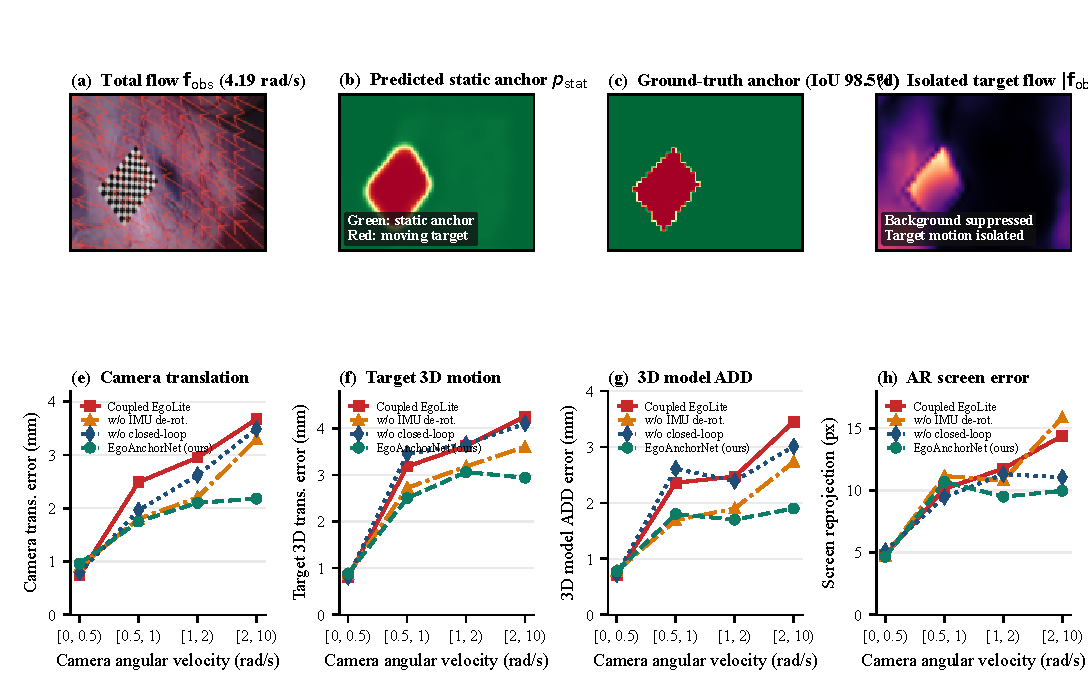
\includegraphics[width=\textwidth]{fig4_ego_anchor_net.pdf}
\caption{EgoAnchorNet qualitative static-anchor disentanglement and quantitative ablation across $260$ validation pairs. \textbf{(a)} Input frame at $4.19$~rad/s overlaid with total observed flow $\mathbf{f}_{\text{obs}}$. \textbf{(b)} Predicted static-anchor probability $p_{\text{stat}}$ (green: stationary background anchor; red: moving target). \textbf{(c)} Ground-truth static-anchor mask ($98.5\%$ IoU). \textbf{(d)} Isolated target motion magnitude $\|\mathbf{f}_{\text{obs}} - \mathbf{f}_{\text{cam}}\|$ after subtracting solved 3D camera ego-motion flow; background motion is suppressed. \textbf{(e)--(h)} Median camera translation error (mm), target 3D translation error (mm), 3D model ADD error (mm), and screen reprojection error (px at $1280\times720$) across four angular-velocity bins for Coupled EgoLite, EgoAnchorNet w/o IMU de-rotation, EgoAnchorNet w/o closed-loop refinement, and EgoAnchorNet (full).}
\label{fig:ego_anchor}
\end{figure*}

\begin{table*}[!t]
\centering
\caption{EgoAnchorNet Component Ablation on the Hybrid Dual-Motion Validation Corpus ($260$ Pairs Across Four Angular-Velocity Bins: $n=10$ in $\mathcal{B}_1$, $n=38$ in $\mathcal{B}_2$, $n=106$ in $\mathcal{B}_3$, $n=106$ in $\mathcal{B}_4$; Medians Reported).}
\label{tab:ego_anchor}
\renewcommand{\arraystretch}{1.12}
\resizebox{\textwidth}{!}{%
\begin{tabular}{llcccccc}
\toprule
\textbf{Metric} & \textbf{Model Variant} & \textbf{$[0.0, 0.5)$ rad/s} & \textbf{$[0.5, 1.0)$ rad/s} & \textbf{$[1.0, 2.0)$ rad/s} & \textbf{$[2.0, 10.0)$ rad/s} & \textbf{Fast-Bin Gain} \\
\midrule
\multirow{4}{*}{\textbf{Camera Trans. Error (mm)}}
 & Coupled EgoLite (No Anchor Gate, Single $\mathrm{SE}(3)$) & \textbf{0.74} & 2.49 & 2.95 & 3.67 & Baseline \\
 & EgoAnchorNet w/o IMU De-Rotation Prior & 0.89 & 1.80 & 2.20 & 3.30 & $-10.1\%$ \\
 & EgoAnchorNet w/o Closed-Loop Refinement & 0.79 & 1.96 & 2.62 & 3.49 & $-4.9\%$ \\
 & \textbf{EgoAnchorNet Full (Ours)} & 0.96 & \textbf{1.75} & \textbf{2.10} & \textbf{2.18} & \textbf{$-40.6\%$} \\
\midrule
\multirow{4}{*}{\textbf{Target 3D Trans. Error (mm)}}
 & Coupled EgoLite (No Anchor Gate, Single $\mathrm{SE}(3)$) & \textbf{0.81} & 3.18 & 3.62 & 4.25 & Baseline \\
 & EgoAnchorNet w/o IMU De-Rotation Prior & 0.87 & 2.72 & 3.18 & 3.60 & $-15.3\%$ \\
 & EgoAnchorNet w/o Closed-Loop Refinement & \textbf{0.81} & 3.45 & 3.66 & 4.10 & $-3.5\%$ \\
 & \textbf{EgoAnchorNet Full (Ours)} & 0.88 & \textbf{2.50} & \textbf{3.06} & \textbf{2.94} & \textbf{$-30.8\%$} \\
\midrule
\multirow{4}{*}{\textbf{3D Model ADD Error (mm)}}
 & Coupled EgoLite (No Anchor Gate, Single $\mathrm{SE}(3)$) & \textbf{0.71} & 2.36 & 2.47 & 3.45 & Baseline \\
 & EgoAnchorNet w/o IMU De-Rotation Prior & 0.78 & \textbf{1.69} & 1.90 & 2.73 & $-20.9\%$ \\
 & EgoAnchorNet w/o Closed-Loop Refinement & 0.72 & 2.61 & 2.39 & 3.01 & $-12.8\%$ \\
 & \textbf{EgoAnchorNet Full (Ours)} & 0.78 & 1.80 & \textbf{1.70} & \textbf{1.90} & \textbf{$-44.9\%$} \\
\midrule
\multirow{4}{*}{\textbf{AR Screen Reprojection (px)}}
 & Coupled EgoLite (No Anchor Gate, Single $\mathrm{SE}(3)$) & 4.83 & 10.12 & 11.75 & 14.40 & Baseline \\
 & EgoAnchorNet w/o IMU De-Rotation Prior & 4.71 & 11.16 & 10.81 & 15.87 & $+10.2\%$ \\
 & EgoAnchorNet w/o Closed-Loop Refinement & 5.13 & \textbf{9.47} & 11.31 & 11.05 & $-23.3\%$ \\
 & \textbf{EgoAnchorNet Full (Ours)} & \textbf{4.66} & 10.69 & \textbf{9.50} & \textbf{9.97} & \textbf{$-30.8\%$} \\
\midrule
\multirow{2}{*}{\textbf{Region Segmentation IoU (\%)}}
 & Static-Anchor Region $\mathcal{M}_{\text{stat}}$ IoU (\%) & 98.99 & 99.01 & 99.18 & 99.08 & --- \\
 & Independently Moving Target $\mathcal{M}_{\text{obj}}$ IoU (\%) & 86.92 & 89.72 & 90.10 & 88.89 & --- \\
\bottomrule
\end{tabular}%
}
\end{table*}

\subsection{EgoAnchorNet Component Ablation on 260 Validation Pairs}
Fig.~\ref{fig:ego_anchor} and Table~\ref{tab:ego_anchor} evaluate EgoAnchorNet on the $260$ validation pairs of the hybrid dual-motion corpus:
\begin{enumerate}
    \item \textbf{Static-Anchor vs. Moving-Target Disentanglement:} Across all four angular-velocity bins, EgoAnchorNet segments stationary background anchors $\mathcal{M}_{\text{stat}}$ with $98.99\%\text{--}99.18\%$ IoU and the independently moving target $\mathcal{M}_{\text{obj}}$ with $86.92\%\text{--}90.10\%$ IoU. On the $4.19$~rad/s sample in Fig.~\ref{fig:ego_anchor}(a)--(d), subtracting the solved 3D camera flow $\mathbf{f}_{\text{cam}}$ suppresses background flow and isolates the target's own motion field $\|\mathbf{f}_{\text{obs}} - \mathbf{f}_{\text{cam}}\|$.
    \item \textbf{Camera Ego-Motion Precision:} In the fastest bin ($[2.0,10.0)$~rad/s, $n=106$), Coupled EgoLite (which lacks static-anchor gating and IMU de-rotation) suffers $0.21^\circ$ rotation error and $3.67$~mm camera translation error because moving target pixels bias the camera Gauss--Newton update. EgoAnchorNet reduces fast-bin camera rotation error to $0.08^\circ$ and camera translation error to $2.18$~mm ($-40.6\%$).
    \item \textbf{Target 3D Motion and End-to-End Registration:} Solving the second Gauss--Newton update on the camera-subtracted residual flow reduces fast-bin target 3D translation error from $4.25$~mm (Coupled EgoLite) to $2.94$~mm ($-30.8\%$), 3D model ADD error from $3.45$~mm to $1.90$~mm ($-44.9\%$), and $1280\times720$ screen reprojection error from $14.40$~px to $9.97$~px ($-30.8\%$). Removing either the IMU de-rotation prior ($2.73$~mm ADD, $15.87$~px) or the closed-loop dual residual refinement ($3.01$~mm ADD, $11.05$~px) degrades high-rate registration accuracy.
\end{enumerate}

\begin{figure*}[!t]
\centering
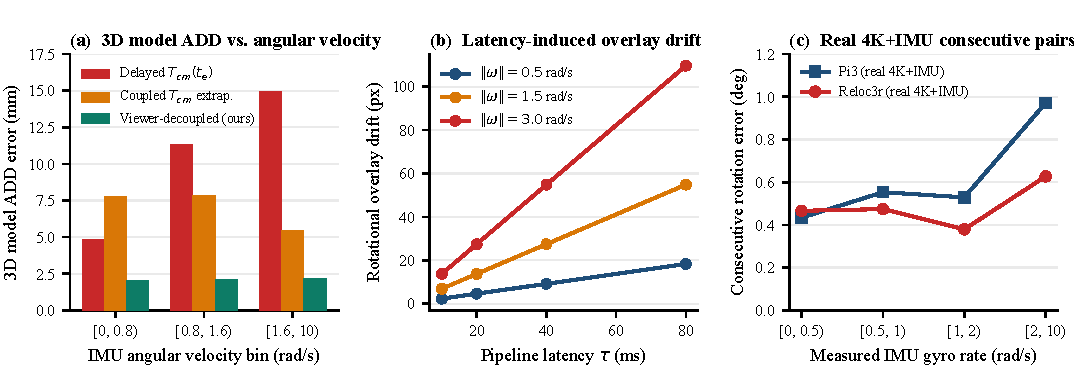
\includegraphics[width=\textwidth]{fig3_add_and_real_bins.pdf}
\caption{3D model ADD error, latency sweep, and real 4K+IMU consecutive-frame evaluation. \textbf{(a)} 3D model ADD error (mm) across IMU angular-velocity bins at $\tau = 60$~ms delay ($89$ frames, $\sigma_{\text{px}}=1.2$~px). \textbf{(b)} Rotational overlay drift (px) vs. pipeline delay $\tau$ and angular rate $\|\boldsymbol{\omega}\|$. \textbf{(c)} Consecutive-frame rotation error of Pi3~\cite{wang2025pi3} and Reloc3r~\cite{dong2025reloc3r} on three real 4K+IMU sessions ($48$ pairs, $12$ per bin).}
\label{fig:add_real}
\end{figure*}

\begin{table}[!t]
\centering
\caption{3D Model Registration Error (ADD in mm and Screen Reprojection in px) at $\tau = 60$~ms Pipeline Delay ($89$ Frames, $30$~fps, $\sigma_{\text{px}}=1.2$~px).}
\label{tab:add}
\renewcommand{\arraystretch}{1.15}
\setlength{\tabcolsep}{3.5pt}
\begin{tabular}{lcccc}
\toprule
\textbf{Strategy} & \textbf{$[0, 0.8)$} & \textbf{$[0.8, 1.6)$} & \textbf{$[1.6, 10)$} & \textbf{Reproj.} \\
 & ($n=63$) & ($n=11$) & ($n=15$) & \textbf{(px)} \\
\midrule
Delayed $T_{cm}(t_e)$ & 4.86 mm & 11.34 mm & 14.94 mm & 3.63 \\
Coupled $T_{cm}$ Extrap. & 7.76 mm & 7.82 mm & 5.46 mm & \textbf{1.51} \\
\textbf{Viewer-Decoupled} & \textbf{2.03 mm} & \textbf{2.07 mm} & \textbf{2.19 mm} & 1.55 \\
\bottomrule
\end{tabular}
\end{table}

\subsection{Stage-II Latency Compensation and Real 4K+IMU Sessions}
Table~\ref{tab:add} and Fig.~\ref{fig:add_real}(a) test our Stage-II display update on a $40$~mm 3D navigation target along an orbit-plus-fast-yaw trajectory ($\tau = 60$~ms, $89$ frames, $30$~fps, $\sigma_{\text{px}}=1.2$~px). Rendering with the exposure-time pose $T_{cm}(t_e)$ increases 3D model ADD from $4.86$~mm at $<0.8$~rad/s to $14.94$~mm at $\ge 1.6$~rad/s. Extrapolating the composite pose $T_{cm}$ lowers 2D reprojection error to $1.51$~px but corrupts 3D model position across all bins ($7.76$~mm slow, $5.46$~mm fast). Decoupling viewer motion keeps 3D ADD at $2.03\text{--}2.19$~mm across all bins with $1.55$~px reprojection error.

Fig.~\ref{fig:add_real}(c) evaluates consecutive $30$~fps frames from three real 4K camera + $200$~Hz IMU sessions (\texttt{gtraj\_20261002\_002134}, \texttt{003129}, and \texttt{024309}, $48$ pairs, $12$ per gyro bin). Whereas uniform 64-frame subsampling placed $134$ of $189$ pairs into $[2.0,10.0)$~rad/s, consecutive-frame sampling across all four gyro bins shows rotation error rising in $[2.0,10.0)$~rad/s from $0.434^\circ$ to $0.971^\circ$ for Pi3 and from $0.466^\circ$ to $0.627^\circ$ for Reloc3r.

\section{Limitations}
\begin{enumerate}
    \item \emph{No optical see-through HMD:} All experiments render overlays onto 4K or stereo video frames; optical combiner calibration and pupil swim are outside our scope.
    \item \emph{Metric scale source:} Monocular 4K millimetre error relies on a known $3.0$~mm target grid, and the $46.5$~mm stereo baseline in simulation must be replaced by per-scope stereo calibration in wet-lab trials.
    \item \emph{Rolling shutter and soft-tissue deformation:} Our update acts at frame exposure midpoints and models rigid target increments; high-frequency rolling-shutter row skew and non-rigid tissue peristalsis require row-timed readout warps and deformable surface tracking.
\end{enumerate}

\section{Conclusion}
Under simultaneous camera and target motion, viewer ego-motion drives feature loss, tracking failure, target-ROI pose error, and latency-induced overlay drift. By using IMU-guided de-rotation to isolate stationary scene anchors, solving camera ego-motion and target 3D motion in cascaded Gauss--Newton stages, and propagating only the viewer pose over the pipeline delay at display time, our method keeps 3D model ADD at $1.79\text{--}2.19$~mm and removes $75.8\%$ of high-rate AR overlay shift.

\section*{Data and Code Availability}
The evaluation protocol, three-condition counterfactual benchmark summaries, figure generation scripts, and LaTeX manuscript sources are publicly available at \url{https://github.com/liranyang123456-commits/Viewer-Decoupled-3D-Registration}, with the dual-motion simulator and real 4K+IMU capture tools hosted at \url{https://github.com/liranyang123456-commits/EGO_Mo}.

\bibliographystyle{IEEEtran}
\bibliography{refs}

\begin{IEEEbiographynophoto}{Ranyang Li}
is with the School of Artificial Intelligence and Big Data, Henan University of Technology, Zhengzhou, China. His research interests include mixed reality spatial registration, visual-inertial navigation, and medical image computing.
\end{IEEEbiographynophoto}

\begin{IEEEbiographynophoto}{Nan Wei}
is with Henan Provincial People's Hospital, Zhengzhou University, Zhengzhou, China. Her research interests include image-guided intervention and clinical navigation systems.
\end{IEEEbiographynophoto}

\begin{IEEEbiographynophoto}{Zhipeng Lin}
is with the State Key Laboratory of Virtual Reality Technology and Systems, Beihang University, Beijing, China. His research interests include augmented reality, computer graphics, and surgical simulation.
\end{IEEEbiographynophoto}

\begin{IEEEbiographynophoto}{Wufeng Liu}
is with the School of Artificial Intelligence and Big Data, Henan University of Technology, Zhengzhou, China. His research interests include computer vision and 3D scene reconstruction.
\end{IEEEbiographynophoto}

\begin{IEEEbiographynophoto}{Chao Fan}
is with the School of Artificial Intelligence and Big Data, Henan University of Technology, Zhengzhou, China. His research interests include intelligent sensing and multi-sensor fusion.
\end{IEEEbiographynophoto}

\begin{IEEEbiographynophoto}{Junjun Pan}
is a Professor with the State Key Laboratory of Virtual Reality Technology and Systems, Beihang University, Beijing, China. His research interests include virtual reality, augmented reality, computer graphics, and medical simulation.
\end{IEEEbiographynophoto}

\end{document}
